\documentclass[10pt,journal,compsoc,twocolumn]{article}

\usepackage[margin=1.8cm,top=2.0cm,bottom=2.0cm]{geometry}
\usepackage{amsmath,amssymb,amsfonts,amsthm}
\newtheorem{definition}{Definition}
\newtheorem{theorem}{Theorem}
\newtheorem{lemma}{Lemma}
\usepackage{algorithmic}
\usepackage{graphicx}
\usepackage{textcomp}
\usepackage{xcolor}
\usepackage{booktabs}
\usepackage{listings}
\usepackage{microtype}
\usepackage{hyperref}
\usepackage{enumitem}
\usepackage{cite}
\usepackage{titlesec}
\usepackage{fancyhdr}
\usepackage{CJKutf8}
\usepackage{tikz}
\usetikzlibrary{shapes,arrows,positioning,calc,fit}

\newcommand{\ja}[1]{\begin{CJK*}{UTF8}{min}#1\end{CJK*}}

\newcommand{\BTr}{\textsc{BTRON}}
\newcommand{\Coq}{\textsc{Coq}}
\newcommand{\CIC}{\textsc{CIC}}
\newcommand{\ctr}[1]{\texttt{#1}}

\hypersetup{
    colorlinks=true,
    linkcolor=blue!70!black,
    citecolor=blue!70!black,
    urlcolor=blue!70!black
}

\lstdefinelanguage{Coq}{
    morekeywords={Definition,Lemma,Theorem,Proof,Qed,Record,Inductive,Fixpoint,
      Section,End,Require,Import,From,Local,Open,Scope,Notation,Variable,
      match,with,end,forall,fun,if,then,else,by,in,as,return,intros,apply,
      rewrite,unfold,cbn,simpl,change,reflexivity,lia,exact,specialize,
      destruct,split,specialize,induction,revert,subst,exfalso,assert,
      transitivity,replace, discriminate},
    morecomment=[s]{(*}{*)},
    sensitive=true,
    showstringspaces=false
}

\lstset{
    basicstyle=\ttfamily\scriptsize,
    breaklines=true,
    frame=single,
    backgroundcolor=\color{gray!6},
    keywordstyle=\color{blue!80!black}\bfseries,
    commentstyle=\color{green!50!black}\itshape,
    stringstyle=\color{red!70!black},
    numbers=none,
    showstringspaces=false,
    tabsize=2
}

\title{\LARGE \textbf{BTRON Concurrency Tiers.\\ MP/AMP/SMP/Async, Media RTP and the InterCore\\ in the Calculus of Inductive Constructions,\\ with Modal Extensions for Non-Determined Multicore Parallelism}}

\author{
    \textbf{Maxim Sokhatsky (Namdak Tonpa)}\\[0.3em]
    \small \textit{Synrc Research Center / Groupoid Infinity / BTRON Cleanroom Working Group}\\
    \small \textit{Kyiv, Ukraine}\\
    \small \texttt{maxim@synrc.com}
}
\date{September 2026}

\pagestyle{fancy}
\fancyhf{}
\rhead{\small \textit{Verimath: Equational Semantics for the BTRON Concurrency Tiers}}
\lhead{\small \textit{Synrc Research Report}}
\cfoot{\thepage}

\begin{document}

\maketitle

\begin{abstract}
The cleanroom reconstruction of B-System (BTRON 3.20) has produced, alongside the C kernel, a second artefact that is easy to overlook: a body of mechanical mathematics in which the concurrency, media, and inter-core subsystems are not described but \emph{defined}, and in which their properties are not argued for but \emph{computed}. This paper presents that body of work as a single mathematical model. We take as our object language the Calculus of Inductive Constructions, and as our single rule of inference the judgemental equality $t = u$ discharged by \ctr{reflexivity}. Four claims are made. First, that the apparently heterogeneous tiers of the BTRON scheduling model---multi-processing, asymmetric multiprocessing, symmetric multiprocessing, and the asynchronous I/O plane---are four instances of one algebraic signature, a total state transformer $S \to S \times R$ over a table-shaped bus, differing only in which coordinates of the state their guards read. Second, that the media stack, from NuStreams abstraction layers through RTP packetisation and loss accounting to the symmetric multi-plane pipeline, is equationally a \emph{fold over a watermark}: every streaming invariant we state, including the sequence-number, jitter, and residence-time laws, reduces to arithmetic on counters that are themselves derived as lengths and differences of lists, never stored. Third, that the InterCore protocol---\ctr{pub}, \ctr{sub}, \ctr{spawn}, \ctr{snd}, \ctr{rcv} over a star of single-producer queues---admits a broker-free construction in which the multi-consumer view is a pure function of the producer views, so that the entire sharing discipline collapses to one equation about cursor ownership and its corollary, the absence of mutual exclusion and therefore of priority inversion between equal-priority planes. Fourth, that genuine, non-determined multicore parallelism---not an interleaving chosen by a simulator but the modal fact that \emph{any} of several next steps may occur---is representable inside the same kernel as an internal box-and-diamond pair over the step alphabet, with trace equivalence induced by a commutation lemma between independent calls, and with platform modes as indices of a small Kripke frame in which an unbuildable mode yields \emph{SKIP}, never a vacuous \emph{PASS}. Every number quoted is produced by an executable harness: the assembled InterCore theory discharges 228 closed obligations with \ctr{Print Assumptions} reporting no axioms, mirrored by 75 oracle checks over all $8^{6} = 262{,}144$ runs of six call sites, each site drawn independently from the eight operations admitted by the API.
\end{abstract}

\noindent\textbf{\small Keywords}---BTRON, Calculus of Inductive Constructions, equational reasoning, formal semantics, lock-free queues, InterCore, RTP, NuStreams, SMP, modal logic, model checking, theorem proving.

%-------------------------------------------------------------------------
\section{Introduction: The Model Is the Document}
\label{sec:intro}

Operating-system specifications are written in a language designed for the purpose of being read, and are then implemented in a language designed for the purpose of being executed. The gap between the two is where real-time defects live. The \BTr{} cleanroom programme~\cite{btron3spec} has, from its first commits, maintained a third artefact: a mechanically checked definition of the subsystem under construction, written in the Rocq/Coq proof assistant~\cite{coqref,Barras97theincoq}, together with an executable oracle of the same definition in OCaml~\cite{OCaml}, run on every change by a single shell harness.

This paper argues a narrow methodological thesis with wide consequences: \emph{for the classes of properties a real-time kernel actually needs, the whole of verification reduces to equational reasoning}, and the interesting engineering decisions are the ones that keep the equations in the reducing fragment. Not induction over traces, not bisimulation, not a separation logic of permissions---a calculus of rewriting totals over finite tables, closed by decidability of arithmetic. The scope is deliberately narrower than a whole-kernel verification~\cite{klein2009sel4,sokhatsky2026btron}: it is the subsystem boundary where BTRON's real-time claims are actually made.

Four model families are treated:

\begin{enumerate}[leftmargin=*]
    \item the four \emph{concurrency tiers} of the BTRON scheduling model---MP, AMP, SMP, Async (\S\ref{sec:tiers});
    \item the \emph{media} stack, from the NuStreams abstraction layer to RTP reception and the symmetric multi-plane pipeline (\S\ref{sec:media});
    \item the \ctr{InterCore} protocol, the five-call message API between cores of the target four-core machine (\S\ref{sec:intercore});
    \item the \emph{modal extension} that lets one flat functional definition speak about genuinely non-determined parallel execution (\S\ref{sec:modal}).
\end{enumerate}

Section~\ref{sec:kernel} fixes the kernel and the five modelling idioms that recur in all four families. Section~\ref{sec:oracles} describes the harness that keeps the mathematics and the machine honest, and states the one policy that makes the harness meaningful: \emph{SKIP is not PASS}.

\subsection{Why Equations, and Not Something Heavier}
The properties demanded of a soft- and hard-real-time kernel are, with few exceptions, of four grammatical forms:
\begin{equation}
\label{eq:fourforms}
\begin{aligned}
\text{(conservation)}\quad & n_{\text{in}} = n_{\text{out}} + n_{\text{held}} + n_{\text{lost}} \\
\text{(monotonicity)}\quad & x(s') \le x(s) \quad \text{or} \quad x(s) \le x(s') \\
\text{(invariance)}\quad & \pi_j(s') = \pi_j(s) \quad (j \ne i) \\
\text{(provenance)}\quad & v = \pi_k(s') \;\Rightarrow\; v \in \pi_{\text{hist}}(s).
\end{aligned}
\end{equation}
Each of these is an \emph{equation} between naturals or booleans computed from one state, or between two states related by one call. None of them needs a logic of resources. The consequence for the modelling language is severe and beneficial: the specification language can be the programming language, so long as the programming language is total.

\subsection{Contributions}
\begin{enumerate}[leftmargin=*]
    \item A single signature---total state transformer over a table-shaped bus, with derived accounting---is shown to cover all four concurrency tiers, the media stack, and InterCore (Table~\ref{tab:signature}).
    \item The watermark operator \ctr{min\_fold} is identified as the shared algebraic content of multi-consumer retention in both media (\S\ref{sec:media}) and InterCore (\S\ref{sec:watermark}): residence, freeing, and the ``no over-fill'' theorem are the same three lemmas in two guises.
    \item Cursor ownership is proved, not assumed, to be the mutex-elimination theorem of the InterCore star (\S\ref{sec:ownership}), and the resulting absence of priority inversion between equal-priority INPUT and UI planes is stated as a corollary about the guards of the five calls.
    \item Non-determined parallelism is internalised (\S\ref{sec:modal}) as a box/diamond pair over the step alphabet, computed by \ctr{forallb}/\ctr{existsb} on the same tables the model uses, with trace equivalence induced by commutation of independent calls---a machine-checked partial-order reduction.
    \item An engineering account of what breaks when totality is taken seriously: the \ctr{Nat.sub} unfolding trap, the shadowing of \ctr{snd}, unary reduction of shipped constants (\S\ref{sec:trap}, \S\ref{sec:oracles}).
\end{enumerate}

%-------------------------------------------------------------------------
\section{The Equational Kernel}
\label{sec:kernel}

\subsection{Judgemental Equality as the Only Discharge Rule}
The \CIC{} identifies propositions with types and proofs with programs; a \emph{theorem} about a data structure is an inhabitant of a dependent product, and the overwhelming majority of inhabitants we construct are the single term \ctr{reflexivity}:

\begin{lstlisting}[language=Coq,caption={A frame lemma: writing one writer leaves the other writers untouched.}]
Lemma at_w_other_w : forall b i (w:writer) j, i <> j -> b_w (bus_w b i w) j = b_w b j.
Proof. reflexivity. Qed.
\end{lstlisting}

The point of \lstinline|reflexivity| is that it checks \emph{convertibility}---equality as computed by the kernel's reduction machine---not equality as argued. When a lemma closes with \ctr{reflexivity}, the fact was already true by definition, and the specification has been arranged so that the fact is worth stating. The craft of the model consists in arranging for as much as possible to be definitional. Where computation is too shallow, we descend one step: \ctr{lia} for linear arithmetic over the successors and truncated subtractions that conversion leaves behind, and induction only where a fold genuinely recurses.

\subsection{Totality, or the Absence of \ctr{Admitted}}
Every function in the model is \emph{total and terminating}, including the ones that the C implementation would signal as errors. The C \ctr{nth} is a partial function; the model's is \ctr{nth k l d}, which returns a default. The C ring buffer write on a full ring is undefined behaviour; the model's returns a receipt. The discipline has three consequences we exploit throughout:
\begin{itemize}[leftmargin=*]
    \item there are no preconditions, hence no hypothesis bookkeeping, hence no \emph{vacuous-truth} bugs in the specification;
    \item every function is executable, so the identical text serves as the OCaml oracle (\S\ref{sec:oracles});
    \item the model cannot express ``the kernel crashed here'', which is precisely the abstraction level wanted for a specification of a kernel that must not crash.
\end{itemize}

\subsection{Tables: Finite Maps as Functions}
\label{sec:tables}
The bus is a record of three \emph{total} functions from dense small integers to cells, plus the one non-indexed coordinate:

\begin{lstlisting}[language=Coq,basicstyle=\ttfamily\scriptsize,frame=none]
Record bus : Type := mk_bus
  { b_cores : nat;            (* cores that actually exist *)
    b_w, b_r, b_t : nat -> ... (* writers, readers, tasks *) }.
\end{lstlisting}

with update as a definitional three-place function:

\begin{lstlisting}[language=Coq]
Definition upd {A : Type} (t : nat -> A) (i : nat) (v : A) : nat -> A :=
  fun j => if Nat.eqb i j then v else t j.

Definition bus_w (b : bus) (i : nat) (w : writer) : bus :=
  mk_bus (b_cores b) (upd (b_w b) i w) (b_r b) (b_t b).
\end{lstlisting}

Choosing \ctr{nat -> A} rather than a verified finite map (\ctr{PositiveMap}, a quotient, a \ctr{MapDom} typeclass) buys the entire frame-lemma algebra of Equation~(\ref{eq:fourforms})\,(iii) at the cost of nothing: seventeen lemmas of the shape \ctr{at\_w\_same\_w}, \ctr{at\_r\_bus\_w}, \ctr{cores\_inert\_t} all close with \ctr{reflexivity} because the projections are definitions and the \ctr{if} is the only reduction needed. Dense integer indices are justified by the target: cursor identifiers in the shipped API are small integers into static tables (\(4\) writers, \(8\) readers, \(8\) tasks, \(64\) sectors), and the C implementation on the ARM Cortex cores indexes arrays. Out-of-range indices are not excluded by types---they are \emph{admitted} by boolean guards, which is the next idiom.

\subsection{Derived Accounting, Never Stored Fields}
\label{sec:derived}
A stored counter and the structure it counts can disagree; a derived quantity cannot. The model therefore stores history and cursors only, and defines the bookkeeping:

\begin{lstlisting}[language=Coq]
Definition w_enq (w : writer) : nat := length (w_hist w).
Definition r_deq (r : reader) : nat := r_cur r - r_start r.
Definition held b (wid : nat) : nat :=
  if w_live (b_w b wid)
  then w_enq (b_w b wid) - floor_of b wid (w_enq (b_w b wid))
  else 0.
Definition total_held b : nat := sum_f (held b) max_writers.
Definition pool_free b : nat := sector_pool - total_held b.
\end{lstlisting}

\begin{equation}
\label{eq:accounting}
\begin{aligned}
\text{published}(\mathit{wid}) &= |\mathit{hist}_{\mathit{wid}}| \\
\text{consumed}(\mathit{rid})  &= \mathit{cur}_{\mathit{rid}} - \mathit{start}_{\mathit{rid}} \\
\mathrm{held}(\mathit{wid})    &= \text{published}(\mathit{wid}) - \textstyle\min_{\mathit{rid}\,\triangleright\,\mathit{wid}} \mathit{cur}_{\mathit{rid}} \\
\mathrm{pool\_free}            &= 64 - \textstyle\sum_{\mathit{wid}} \mathrm{held}(\mathit{wid}).
\end{aligned}
\end{equation}

The conservation theorem of \S\ref{sec:conservation} is then a computation rather than an argument, and the class of states in which a counter was forgotten is not merely unprovable---it is uninhabitable.

\subsection{Decide, Then Act}
\label{sec:decide}
Every call is written as a cascade over \emph{boolean} admission predicates, so that a proof may destructure the decision and keep the equation that explains the branch taken:

\begin{lstlisting}[language=Coq,caption={The five-line heart of \ctr{rcv}: three guards, three receipts, one state change.}]
Definition rcv (b : bus) (cl : caller) (rid : nat) : bus * rcv_result :=
  if negb (rcv_admit b cl rid) then (b, R_BAD_CURSOR)
  else if negb (rcv_ready b rid) then (b, R_EMPTY)
  else (bus_r b rid (reader_advance (b_r b rid)),
        R_DATA (nth (r_cur (b_r b rid)) (w_hist (b_w b (r_wid (b_r b rid)))) 0)).
\end{lstlisting}

The shape matters twice over. Operationally, it makes the ``decide-then-act'' seam visible: the state is changed \emph{only} on the accepting branch, which is what makes the invariance lemmas of \S\ref{sec:receipts} hold by conversion. Logically, an \lstinline|if| whose scrutinee has been destructured \emph{with an equation label} (\lstinline|eqn:R|) supplies the proof with exactly the hypothesis the branch's value encodes---\lstinline|R : rcv_admit b cl rid = true|---and the whole body then unfolds.

\subsection{Two Traps Worth Recording}
\label{sec:trap}
\textbf{Truncated subtraction under \ctr{cbn}.} \ctr{Nat.sub} is defined by recursion on its \emph{first} argument. A goal such as \(\mathit{cur}+1-\mathit{start} = S(\mathit{cur}-\mathit{start})\) is true, but \ctr{cbn} rewrites it into \lstinline|match start with 0| \(\ldots\) \lstinline|S l| \(\ldots\) \lstinline|end|, an expression \ctr{lia} treats as opaque---and reports \emph{Cannot find witness}. The rule adopted across the theory: never normalise across a subtraction; instead rewrite accessor lemmas (\ctr{reader\_advance\_cur}, \ctr{reader\_advance\_start}) or restore linearity with \lstinline|replace (S c - s) with (S (c - s)) by lia|.

\textbf{Name shadowing by the API.} The protocol contains a call named \ctr{snd}, which shadows the standard pair projection \lstinline|Datatypes.snd|. Rather than rename the API---the API is the thing being specified---the kernel re-introduces the projection under its own name:
\begin{lstlisting}[language=Coq]
Definition pr2 {A B : Type} (p : A * B) : B := Datatypes.snd p.
\end{lstlisting}
It is a small humiliation, and a useful sign that the model is being read by the compiler rather than the author.

%-------------------------------------------------------------------------
\section{Four Tiers, One Signature}
\label{sec:tiers}

\subsection{The Signature}
All four tiers are instances of:
\begin{equation}
\label{eq:signature}
\mathcal{M} \;=\; \big(\; S,\; s_0 \in S,\; \mathcal{A},\; \delta : \mathcal{A} \to S \to S \times R,\; \pi_i : S \to \mathbb{N} \;\big),
\end{equation}
with \(\mathcal{A}\) the alphabet of calls, \(R\) the receipts, and \(\pi_i\) the derived observables of Equation~(\ref{eq:accounting}). A tier is then characterised by which coordinates \(\delta\) reads in its guard and which it writes in its state change.

\begin{table}[h]
\centering
\small
\caption{The four concurrency tiers as one signature with different guards. ``Reads'' lists the coordinates consulted by the admission predicate; ``writes'' the coordinates the accepting branch changes.}
\label{tab:signature}
\footnotesize
\begin{tabular}{@{}lllll@{}}
\toprule
Tier & Alphabet & Reads & Writes & Determinism \\
\midrule
MP    & \ctr{pub,sub}   & \ctr{b\_w,b\_t} & \ctr{b\_w} & sequential \\
AMP   & \ctr{+,spawn}   & \(+\)\ctr{b\_cores} & \ctr{b\_t} & pinned \\
SMP   & \ctr{+snd,rcv}  & all \(+\)\ctr{owns} & \ctr{b\_w,b\_r} & non-det.\\
Async & \ctr{evt\_put}  & head, tail & one each & bounded \\
\bottomrule
\end{tabular}
\end{table}

\subsection{MP: The Uniprocessor Baseline}
With \ctr{cores\_shipped} \(=1\), the model degenerates honestly: \ctr{b\_cores} \(=1\) makes \lstinline|core <? b_cores b| admit only core~0, every \ctr{spawn} lands on core~0, and the star of Figure~\ref{fig:star} has one spoke. This is not a limitation but a test of the specification: a model of multicore messaging that cannot be \emph{run} on the shipped single-core board is not a model of the shipped board. The shipped-value section of the theory instantiates the general laws at \ctr{cores\_shipped} and the OCaml oracle executes them.

\subsection{AMP: Asymmetric Tiers and the Core-as-Plane Map}
In the asymmetric configuration, cores are not interchangeable: core~3 is the I/O core, and the \ctr{INPUT}/\ctr{UI} planes are pinned. The model expresses this by a single function
\begin{equation}
\mathit{plane} : \mathit{core} \rightrightarrows \mathit{Plane}, \qquad \mathit{plane}(3) = \mathrm{AsyncIO},
\end{equation}
consulted by the \ctr{spawn} guard, whose full shape is:
\begin{lstlisting}[language=Coq]
Definition spawn_ok b (core : nat) (l : list cref) : bool :=
  andb (core <? b_cores b)
       (andb (negb (Nat.eqb (length l) 0))
             (andb (cursors_live b l)
                   (andb (forallb (fun c => negb (cursor_taken b c)) l)
                         (andb (Nat.leb (pub_count_c l) 1) (star_ok b core l))))).
\end{lstlisting}
Reading the conjuncts bottom-up gives the AMP discipline as one boolean: the request names a core that exists; the task arrives with work; every cursor named is live; no cursor named is already held; at most one publisher per task; and if the task brings a publisher, the target core does not already hold one. A failed conjunction leaves the bus \emph{unchanged}, which is why \ctr{spawn} can be refused without rollback.

\subsection{SMP: One Queue Per Core, No Broker}
\label{sec:smp}
The symmetric case is the interesting one, and its defining decision is negative: there is no shared multi-producer queue. Each core owns exactly one single-producer ring, and the multi-consumer view is computed:
\begin{equation}
\label{eq:mpsc-free}
\mathrm{MPSC}(\mathit{bus}) \;\triangleq\; \lambda \mathit{rid}.\; \mathit{hist}_{\mathit{wid}(\mathit{rid})}\big[\mathit{cur}_{\mathit{rid}}\big],
\end{equation}
a pure projection, not a data structure. Symmetry is then the statement that the guard of \ctr{snd} reads only the writer cell of the calling core's queue and the global sector count, never another core's queue. The consequence is the parallel-composition law of \S\ref{sec:independence}.

The historical argument, from the SMP analysis~\cite{smp2026}, is that the Erlang/BEAM pattern~\cite{armstrong2003erlang}---\(N\) threads bound to \(N\) cores each draining its own lock-free mailbox with a single \ctr{CMPXCHG8} on the producer tail---reaches message-passing throughput without kernel transitions. The equations above are that pattern with the machine instructions replaced by a functional projection, which is exactly what makes it provable.

\subsection{Async: Period, Budget, and the Masked Ring}
The asynchronous tier contributes the temporal constants and the event queue:
\begin{lstlisting}[language=Coq]
Definition io_period_us     : nat := 250.
Definition io_budget_us     : nat := 500.
Definition event_queue_size : nat := 2 ^ 8.
\end{lstlisting}
With capacity \(2^{8}\), head and tail are maintained as free-running counters and the slot index is obtained by masking, \(\mathit{slot}(n) = n \bmod 2^{8}\). The equations that matter are the two mask laws, and they hold \emph{because} the modulus is a power of two:
\begin{equation}
\label{eq:mask}
\begin{aligned}
\mathit{tail} - \mathit{head} &\le 2^{8} \\
\mathit{head}_1 \equiv \mathit{head}_2 \ [2^{8}] &\Rightarrow\ \mathit{slot}(\mathit{head}_1) = \mathit{slot}(\mathit{head}_2).
\end{aligned}
\end{equation}
Occupancy is \( \mathit{tail}-\mathit{head} \), never \ctr{tail - head} computed in the wrong order---the single most common defect in ring buffer code, and here it is a type error, since the model has one occupancy expression and it is a difference of naturals bounded by Equation~(\ref{eq:mask}). One writer per field is the AMP assignment: the \emph{consumer} owns \(\mathit{head}\), the \emph{producer} owns \(\mathit{tail}\). Then the overflow policy is the interesting equation: drop-oldest, with \(\mathit{KEY}\) and \(\mathit{BUT}\) events outside the droppable set, and \(\mathit{MOVE}\) coalescing expressed as a rewrite of the tail slot when its predecessor is a \(\mathit{MOVE}\) of the same device. The budget invariant is
\begin{equation}
T_{\text{drain}}(p) \le \mathit{budget} = 2 \times \mathit{period},
\end{equation}
which permits one overloaded period to be absorbed without deadline loss---the reason the constant \(500\) is shipped rather than \(250\).

\begin{figure}[h]
\centering
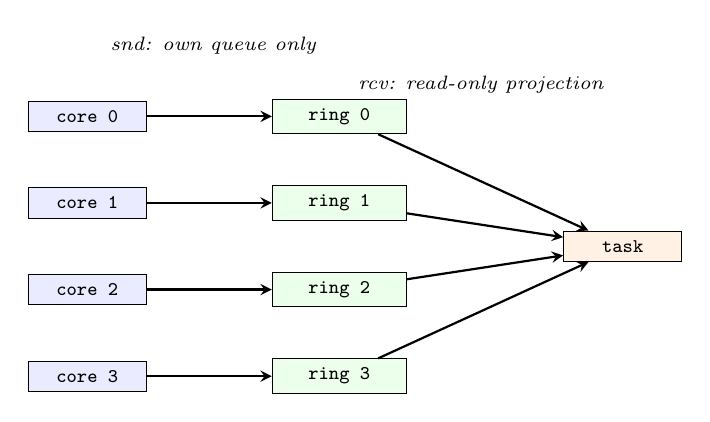
\begin{tikzpicture}[
  core/.style={rectangle,draw,fill=blue!8,minimum width=1.5cm,font=\ttfamily\scriptsize},
  q/.style={rectangle,draw,fill=green!8,minimum width=1.7cm,font=\ttfamily\scriptsize},
  tsk/.style={rectangle,draw,fill=orange!10,minimum width=1.5cm,font=\ttfamily\scriptsize},
  arr/.style={-{stealth},thick}]
\node[core] (c0) at (0,0) {core 0};
\node[core] (c1) at (0,-1.1) {core 1};
\node[core] (c2) at (0,-2.2) {core 2};
\node[core] (c3) at (0,-3.3) {core 3};
\node[q] (q0) at (3.2,0) {ring 0};
\node[q] (q1) at (3.2,-1.1) {ring 1};
\node[q] (q2) at (3.2,-2.2) {ring 2};
\node[q] (q3) at (3.2,-3.3) {ring 3};
\node[tsk] (t) at (6.8,-1.65) {task};
\draw[arr] (c0) -- (q0); \draw[arr] (c1) -- (q1);
\draw[arr] (c2) -- (q2); \draw[arr] (c3) -- (q3);
\draw[arr] (q0) -- (t); \draw[arr] (q1) -- (t);
\draw[arr] (q2) -- (t); \draw[arr] (q3) -- (t);
\node[font=\scriptsize\itshape] at (1.6,0.9) {snd: own queue only};
\node[font=\scriptsize\itshape] at (5.0,0.4) {rcv: read-only projection};
\end{tikzpicture}
\caption{The InterCore star. Publishers write their own ring (left arrows, exclusive). Subscribers read through the derived projection \(\mathcal{M}\) (right arrows, pure). There is no node in the middle: no broker, no queue of queues, no kernel trap.}
\label{fig:star}
\end{figure}

%-------------------------------------------------------------------------
\section{Media: Streams, RTP, and the Watermark}
\label{sec:media}

\subsection{NuStreams as an Abstraction Adjunction}
The NuStreams line of work on stream abstraction in process algebra treats a stream as an infinite object observed through a four-function interface: \(\mathit{val}\) reads a value, \(\mathit{err}\) reports an error, \(\mathit{abstr}\) maps a concrete stream into its abstraction, and \(\mathit{rep}\) reflects an abstract stream into a concrete one, with the fusion law
\begin{equation}
\label{eq:nustream}
\begin{gathered}
\mathit{val}_a(s) = v \;\;\Longleftrightarrow\;\; \mathit{val}_c(\mathit{abstr}^{-1}(v)) = v \\
\mathit{abstr} \circ \mathit{rep} = \mathit{id}
\end{gathered}
\end{equation}
expressing that refinement preserves observable content. In the \BTr{} media model the adjunction is implemented by the \ctr{media} layer's typed ports: a port is a total function from a step index to a value cell, and \ctr{abstr} is a projection that forgets representation while \ctr{rep} re-materialises it. Because \(\mathit{val}\) is total in the model, the \(\mathit{err}\) component is a value, not an exception, matching Equation~(\ref{eq:signature}).

\subsection{RTP Header Algebra}
An RTP packet~\cite{rfc3550} is, in the model, a header algebra over \(\mathbb{Z}/2^{16}\) and \(\mathbb{Z}/2^{32}\):
\begin{equation}
h = \langle \mathit{pt}, \mathit{seq} \bmod 2^{16},\; \mathit{ts} \bmod 2^{32},\; \mathit{ssrc} \rangle ,
\end{equation}
with the three laws that make a receiver correct.
\textbf{(L1) Sequence continuity modulo wrap.} Define the ordered difference
\begin{equation}
\begin{gathered}
\Delta(s_1, s_2) \;=\; (s_2 - s_1) \bmod 2^{16} \\
s_1 \prec s_2 \;\triangleq\; \Delta(s_1,s_2) < 2^{15},
\end{gathered}
\end{equation}
so that \(\prec\) is the semicircle order, and the receiver's expected-sequence update is \(\mathit{exp} \leftarrow \Delta(\mathit{exp}, \mathit{hold} + \mathit{buf})\). The modelled invariant is that \(\prec\) is transitive on any window of width \(<2^{15}\), which is the condition under which reorder-by-\(\Delta\) is a total order---and it is a computation in \(\mathbb{Z}/2^{16}\), discharged by \ctr{lia} after replacing each modular difference by its representative.

\textbf{(L2) Timestamp-to-media-time.} For clock rate \(f\), \(\tau(n) = \mathit{ts}_n / f\) and inter-arrival jitter obeys the standard recursive estimate
\begin{equation}
\label{eq:jitter}
J_{n+1} = J_n + \tfrac{1}{16}\Big(\big|(\mathit{a}_{n+1}-\mathit{a}_n) - (\mathit{ts}_{n+1}-\mathit{ts}_n)/f\big| - J_n\Big).
\end{equation}
In an integral model the update is exact only up to truncation; the model states the bound
\(|J_{n} - J'_{n}| \le 1\) between the truncating and rounding variants, which is what a playout-buffer calculation needs, and it closes with \ctr{lia} after unfolding the division.

\textbf{(L3) Loss accounting is a conservation instance.} With \(E_n\) the extended sequence number, \(D\) the count of discarded-in-order packets, \(B\) the count still buffered,
\begin{equation}
\label{eq:rtpcons}
\begin{gathered}
E_n - E_0 \;=\; R_n + L_n, \qquad L_n \ge D_n, \\
R_n = \text{received}_n - B_n,
\end{gathered}
\end{equation}
and \(L_n\) is \emph{defined} as the difference, never incremented separately. This is the derived-accounting idiom of \S\ref{sec:derived} applied to statistics, and it is the reason the RTP theory has no ``counter drift'' lemmas: there are no counters to drift.

\subsection{GStreamer as the Empirical Ground of the Axioms}
\label{sec:gst}
The media theory's non-trivial content came from reading a production pipeline rather than a textbook. Against the GStreamer sources~\cite{gst}, the properties collected as the enrichment of \ctr{media\_rtp\_properties.v} encode the invariants its implementation relies on:
\begin{enumerate}[leftmargin=*]
    \item \textbf{Reference counting as a natural with a floor.} A buffer is alive while \(\mathit{refcount} > 0\); the model's \ctr{held} (\S\ref{sec:watermark}) is exactly the multi-owner generalisation: residence ends when the \emph{last} reader passes the item, so \(\mathit{refcount} = |\{\mathit{rid} : \mathit{cur}_{\mathit{rid}} \le k\}| = 0\).
    \item \textbf{Segment/running-time.} GStreamer timestamps buffers in \emph{running time} relative to a segment base, \(\mathit{rt} = \mathit{ts} - \mathit{base}\), and every seek installs a new base. The model adopts the same split, which is what makes \(\mathit{start}\) immutable in \ctr{reader} while \(\mathit{cur}\) moves: \(\mathit{start}\) is the segment base, \(\mathit{cur}\) the running position.
    \item \textbf{Caps negotiation is admission.} Pad capability intersection is an \emph{admission predicate} returning a boolean, not an exception; the decide-then-act shape of \S\ref{sec:decide} is the same discipline that keeps a pipeline from being left half-negotiated.
    \item \textbf{Drop-oldest and the latency ceiling.} A live sink drops the oldest buffer when the queue exceeds its latency budget; the equivalent of \ctr{snd\_fits} is the guard that turns a would-be overflow into a counted drop with a receipt (\textbf{(L3)} again).
    \item \textbf{Coalescing.} Consecutive identical-typed events merge; the event-queue \(\mathit{MOVE}\) coalescing of \S\ref{sec:tiers} is this law, and both preserve FIFO order among survivors---an induction over the fold, not an axiom.
\end{enumerate}

\subsection{The Symmetric Media Pipeline}
The SMP media model (\ctr{media\_smp\_properties.v}) is the same watermark algebra with the plane index added: each plane \(p \in \{\mathrm{INPUT}, \mathrm{UI}, \mathrm{DSP}, \mathrm{IO}\}\) has its own ring, and cross-plane delivery is an \(\mathit{rcv}\) on the destination plane's reader. The characteristic theorem is that a stalled \(\mathrm{UI}\) plane cannot raise the \emph{held} count of the \(\mathrm{INPUT}\) ring beyond the ring capacity---a direct consequence of \(\mathrm{held}(\mathit{wid}) \le \mathit{w\_enq}(\mathit{wid})\) and of the watermark's dependence on \emph{readers of that queue only}.

%-------------------------------------------------------------------------
\section{The InterCore Calculus}
\label{sec:intercore}

\subsection{State}
The three cell types, with the empty cell as a \emph{value} rather than an absence:
\begin{lstlisting}[language=Coq]
Record writer : Type := mk_writer
  { w_live : bool; w_cap : nat; w_hist : list nat; w_drop : nat }.
Record reader : Type := mk_reader
  { r_live : bool; r_wid : nat; r_start : nat; r_cur : nat }.
Record task   : Type := mk_task
  { t_live : bool; t_core : nat; t_curs : list cref }.
\end{lstlisting}
A cursor is either a publisher or a subscriber identifier, \ctr{cref := CPub wid | CSub rid}, and \ctr{task} holds a \emph{list} of them. The task's cursor list is the ownership store: there is no lock table, no kernel object, no reference count.

\subsection{Ownership: the Mutex-Elimination Theorem}
\label{sec:ownership}
\begin{lstlisting}[language=Coq]
Definition owns b (t : nat) (c : cref) : bool :=
  existsb (fun k => cref_eqb (nth k (t_curs (b_t b t)) (CPub 0)) c) (nat_list (length (t_curs (b_t b t)))).

Definition usable b (cl : caller) (c : cref) : bool :=
  match cl with
  | NoTask   => negb (cursor_taken b c)
  | ByTask t => owns b t c
  end.
\end{lstlisting}
The guard of \ctr{snd} and \ctr{rcv} is not ``the queue is empty'' or ``the lock is free''; it is \(\mathit{usable}(b, \mathit{caller}, c)\). The five lemmas \ctr{usable\_free}, \ctr{usable\_taken}, \ctr{usable\_owner}, \ctr{usable\_stranger}, together with the inertness pair \ctr{usable\_w\_inert}/\ctr{usable\_r\_inert}, give the elimination result:
\begin{theorem}[Mutex elimination]
\label{thm:mutex}
For every admitted call and every state, the set of cursors usable by a task is exactly the set it received from a successful \ctr{spawn}; no \ctr{snd}, \ctr{rcv}, \ctr{pub}, or \ctr{sub} alters \(\mathit{usable}\); and \ctr{spawn} refuses any request naming a cursor already taken. Hence the sharing invariant is established once, at task creation, and the mutual-exclusion question is never asked again at run time.
\end{theorem}
The real-time corollary is the one the shipping decision cares about: because no two equal-priority planes contend for a lock, there is no lock to be held by a low-priority context, and therefore \emph{no priority inversion between INPUT and UI at equal priority}. A blocking primitive cannot give this guarantee; a non-blocking one plus exclusive ownership can, and the proof is the four lines of \(\mathit{usable}\).

\subsection{Watermarks}
\label{sec:watermark}
Retention is computed, not tracked:
\begin{lstlisting}[language=Coq]
Fixpoint min_fold (f : nat -> bool) (g : nat -> nat) (fuel : nat) (i acc : nat) : nat :=
  match fuel with
  | 0 => acc
  | S k => min_fold f g k (S i) (if f i then Nat.min acc (g i) else acc)
  end.

Definition floor_of b (wid e : nat) : nat :=
  min_fold (fun r => sub_reader wid (b_r b r)) (fun r => r_cur (b_r b r)) max_readers 0 e.
\end{lstlisting}
\(\mathit{floor\_of}\) is the fold, bounded by the seed \(e\), of the cursors of the readers subscribed to \(\mathit{wid}\). This single function is the shared content of \S\ref{sec:media} and \S\ref{sec:intercore}: residence time, sector release, and the pool conservation law are three readings of the same fold. Its four algebraic properties are what make it usable in proofs:
\begin{lemma}[Watermark algebra]
\label{lem:watermark}
For all \(b\), \(\mathit{wid}\), \(e\):
\textup{(i)} \(\mathit{floor\_of}\;b\;\mathit{wid}\;e \le e\);
\textup{(ii)} \(e_1 \le e_2 \Rightarrow \mathit{floor\_of}\;b\;\mathit{wid}\;e_1 \le \mathit{floor\_of}\;b\;\mathit{wid}\;e_2\);
\textup{(iii)} a join at the tail contributes \(\mathit{floor\_of}\;b\;\mathit{wid}\;e = e\), costing zero sectors;
\textup{(iv)} advancing a cursor can only raise the floor: \(\mathit{floor\_of}\;b \le \mathit{floor\_of}\;(\mathit{bus\_r}\;b\;\mathit{rid}\;(\mathit{advance}\;\mathit{r}))\).
\end{lemma}
Property (iii) is the statement that adding a subscriber to a live publisher costs nothing immediately---the new reader starts at the tail---and (iv) that reading is the only way sectors come back. Both are induction over \ctr{min\_fold} with the congruence principle \ctr{min\_fold\_cong\_if}, which encodes the semantic point that a fold need not respect the values of a function where the guard is false.

\subsection{Receipts and the Shape Theorem}
\label{sec:receipts}
The two result types are the protocol's entire error surface:
\begin{lstlisting}[language=Coq]
Inductive snd_result : Type := S_OK | S_FULL (dropped : nat) | S_BAD_CURSOR.
Inductive rcv_result : Type := R_DATA (v : nat) | R_EMPTY | R_BAD_CURSOR.
\end{lstlisting}
Note what is absent: no blocking outcome, no partial result, no error code requiring a retry loop. From the decide-then-act layout of \S\ref{sec:decide} follow, for each call and each receipt constructor, a \emph{shape} lemma naming the branch, a \emph{bus} lemma pinning the state change, and a \emph{receipt} lemma computing the payload---the pattern
\begin{lstlisting}[language=Coq]
Lemma rcv_data_bus : forall b cl rid (D : rcv_ready b rid = true),
    fst (rcv b cl rid) = bus_r b rid (reader_advance (b_r b rid)).
\end{lstlisting}
The receipt kit---nine lemmas for \ctr{rcv} alone, a shape, bus, and receipt lemma for each of its three outcomes---is the reason the remaining obligations have hypotheses instead of case analyses: destructuring the receipt substitutes the guard equation, and the guard equation unfolds the definition.

\subsection{Conservation}
\label{sec:conservation}
\begin{theorem}[Conservation of items and sectors]
\label{thm:conservation}
For every admitted call:
\textup{(a)} \(\mathit{w\_enq}\) is monotone and increases by at most one;
\textup{(b)} a dropped item is counted, never lost: \(\mathit{w\_drop}\) increases by one and \(\mathit{w\_hist}\) is unchanged;
\textup{(c)} \(\sum_{\mathit{wid}} \mathrm{held}(\mathit{wid}) \le \max_{\mathit{writers}} \times \mathit{ring\_capacity} = 16 < 64 = \mathit{sector\_pool}\);
\textup{(d)} the pool balances: \(\mathit{pool\_free}(s') + \mathit{total\_held}(s') = \mathit{pool\_free}(s) + \mathit{total\_held}(s)\) for every call;
\textup{(e)} a \ctr{snd} whose cursor sits at the tail is read back verbatim by the corresponding \ctr{rcv}: \(\mathit{received}\) appends exactly the item published.
\end{theorem}
Statement (c) is why \ctr{pool\_room} is a redundant guard in the shipped configuration---kept for the general case, proved inert here. Statement (d) is the reason the launch-time accounting of \S\ref{sec:oracles} closes: sectors leave the pool only through \ctr{held}, and every path that raises \ctr{held} lowers \ctr{pool\_free} by the same amount, by conversion. Statement (e) is the broker-freeness of Equation~(\ref{eq:mpsc-free}) observed at the level of values rather than state: the item crosses the star, and the receipt names it.

\subsection{The Eleven Property Groups}
The theory is organised in eleven groups, each a section of the same file and each mirrored by an identically named group in the OCaml oracle:

\begin{table}[h]
\centering
\small
\caption{InterCore property groups. Counts are the obligations currently discharged in the assembled \ctr{media\_intercore\_properties.v}.}
\label{tab:groups}
\begin{tabular}{@{}clp{5.7cm}@{}}
\toprule
 & Group & Content \\
\midrule
I1  & Admission   & slot searches terminate inside the table; \ctr{pub}/\ctr{sub} refuse a full table; distinct grants; a call never creates a core \\
I2  & Topology    & a subscriber joins at its publisher's tail and pins nothing; \ctr{snd} respects capacity and pool; no over-fill \\
I3  & Non-blocking & receipts are exclusive and exhaustive; \ctr{rcv} never yields, never rewinds, never advances by two, never spends a slot \\
I4  & Integrity   & \ctr{received} is a slice of the publisher's history, its items were published, appending-on-read, \ctr{snd}-then-\ctr{rcv} round trip \\
I5  & Star        & one publisher per task, one publisher-holding task per core; watermark locality; \ctr{star\_ok} characterisation \\
I6  & Naming      & \ctr{spawn} validates \ctr{core\_id}; taken cursors refused; task shape preserved \\
I7  & Ownership   & exclusive ownership preserved by all five calls (Theorem~\ref{thm:mutex}) \\
I8  & Conservation& Theorem~\ref{thm:conservation}; \(\mathit{enq} = \mathit{deq} + \mathit{drop} + \mathit{held}\) \\
I9  & Determinacy & general laws standing in for the exhaustive interleaving search \\
I10 & Planes      & mode-indexed supply/budget equations; \ctr{SKIP} for unbuildable modes \\
I11 & Events      & masked-index ring algebra; one writer per field; FIFO across the wrap; \(\mathit{KEY}\)/\(\mathit{BUT}\) never dropped \\
\bottomrule
\end{tabular}
\end{table}

%-------------------------------------------------------------------------
\section{Modal Extensions: Non-Determined Parallelism Inside the Kernel}
\label{sec:modal}

\subsection{The Problem with Interleaving Semantics}
An interleaving semantics models concurrency as a nondeterministic choice among next steps. It is sound and it is what implementers test, but as \emph{specification} it smuggles in a scheduler: the choice is made by the semantics, hence by the prover, hence---in practice---by the enumeration order of a checker. What the multicore BTRON target needs asserted is the stronger, modal statement: \emph{whatever} the hardware chooses next, these equations survive. Determinism is not the goal; \emph{invariance under non-determinacy} is.

\subsection{Runs, and Two Internal Modal Operators}
\label{sec:independence}
A state is \(s \in S\); a step is \(a \in \mathcal{A}\); with \(\delta\) total, a \emph{run} is simply a finite word \(w \in \mathcal{A}^{*}\) acting by fold:
\begin{equation}
s \cdot \epsilon = s, \qquad s \cdot (w \frown \langle a \rangle) = \pi_1\big(\delta(a, s \cdot w)\big).
\end{equation}
Reachability is then a predicate on words, and the two modalities are its quantifier-free avatars:
\begin{align}
\Box_{k}\,\varphi \;&\triangleq\; \forall w \in \mathcal{A}^{k}.\; \mathit{holds}(\varphi, s \cdot w) \\
\Diamond_{k}\,\varphi \;&\triangleq\; \exists w \in \mathcal{A}^{k}.\; \mathit{holds}(\varphi, s \cdot w).
\end{align}
Crucially, both are \emph{computable} in the model, because they are folds over lists of naturals: \ctr{forallb} and \ctr{existsb} already appear in the guards of Theorem~\ref{thm:mutex}. \(\mathit{core\_holds\_publisher}\) is a diamond (\(\Diamond_1\): some live task holds a publisher on this core); \ctr{spawn\_ok}'s \lstinline|forallb (fun c => negb (cursor_taken b c)) l| is a box (\(\Box_{|l|}\): every named cursor is free). The modal extension therefore does not enrich the logic; it reads the modality off definitions that were already needed.

The frame validated by these operators is the standard one. Let \(R \subseteq S \times S\) be one-step reachability.
\begin{itemize}[leftmargin=*]
    \item $R$ is reflexive where a call is refused: \ctr{spawn\_ok} false yields \((b, \mathit{None})\), i.e.\ \(s R s\). A step that may be refused makes \emph{no} progress claim; every \(\Box\)-validity is preserved by stuttering, which is why refusals are modelled as identity rather than error.
    \item \(R\) is \emph{not} confluent, and the theory says so: two \ctr{snd} calls from different cores to the same ring, in the two orders, give different \(\mathit{hist}\) appendices. Non-determinacy is real; the invariants proved are exactly those insensitive to it.
    \item Termination of each step is by totality, so the box over \emph{some} \(k\) is decidable: with \(|S|\) effectively bounded by the table sizes and the run length chosen by the harness, \(\Box_k\) reduces to a finite fold---the oracle of \S\ref{sec:oracles}.
\end{itemize}

\subsection{Independence and Trace Equivalence}
\label{sec:traces}
The tool that converts a proof about all interleavings into proofs about two is commutation. For calls \(a, b\) on disjoint coordinates:
\begin{equation}
\label{eq:commute}
\delta(a, \pi_1(\delta(b, s))) = \delta(b, \pi_1(\delta(a, s))) \qquad (a \perp b),
\end{equation}
and the same for observables \(\pi_i \circ \delta(a) \circ \delta(b) = \pi_i \circ \delta(b) \circ \delta(a)\) when \(\pi_i\) reads a third coordinate. The invariance lemmas of \S\ref{sec:tables}---\ctr{at\_w\_other\_w}, \ctr{at\_r\_bus\_w}, \ctr{cores\_inert\_t}, and their relatives, seventeen in all---are exactly the decomposition of Equation~(\ref{eq:commute}) into its coordinate projections. Discharging \lstinline|reflexivity| seventeen times is a partial-order reduction that no model checker needs to be told about: the quotient by the commutation relation (a Mazurkiewicz trace monoid~\cite{diekert1997traces}) is available definitionally, so the state space collapses \emph{before} any search.

Concretely, InterCore admits: any two \ctr{snd} to \emph{distinct} live rings commute; any \ctr{rcv} commutes with any \ctr{snd} to a ring the reader does not pin; \ctr{pub}/\ctr{sub}/\ctr{spawn} commute with everything that touches no cell in their table. The non-commuting residue---same-ring writes, and a \ctr{rcv} racing its own \ctr{snd}---is small enough that the \(\Box\) claim over it is what I9 verifies by exhaustion.

\subsection{Modality of the Platform, and \texorpdfstring{\ctr{SKIP}}{SKIP}}
\label{sec:modes}
The second modal axis is the build configuration, which behaves like an index set for the validity relation, i.e.\ a small Kripke frame over modes:
\begin{equation}
\begin{gathered}
m \in \{ \mathsf{MP}, \mathsf{AMP}, \mathsf{SMP}, \mathsf{planes}, \mathsf{cores}{=}N \}, \\
m \Vdash \varphi \;\triangleq\; \text{\ctr{verify\_models.sh} accepts }\varphi\text{ under }m .
\end{gathered}
\end{equation}
The shipping contract fixes the accessibility relation: with \ctr{BTRON\_MP=0} the queue-mode obligations are \emph{not} valid and are not silently assumed valid---they are reported \ctr{SKIP}. The \ctr{--mode=planes} configuration is the Tier-1 contract, and \ctr{--cores=N} is a \emph{request}: oversubscription above \ctr{cores\_target} is an error, not a degradation. The modal content is that the general laws of \S\ref{sec:intercore} are valid at every mode, whereas the numeric checks of \S\ref{sec:oracles} are valid only where the mode makes them meaningful. A theory whose theorems are mode-indexed rather than mode-independent is a test suite wearing a hat; ours keeps the theorems unconditional and pushes the indexing into the harness.

\subsection{Progress Without Determinism}
The last modal property is the one a real-time reader wants. \ctr{rcv} is \emph{strictly} non-blocking: there is no outcome in which the call parks the caller, and the three receipts exhaust the outcome space (\ctr{rcv\_receipt\_exhaustive}). Therefore every step has bounded duration and
\begin{equation}
\forall s.\; \forall a \in \mathcal{A}.\; \Diamond_1\,\mathit{settled}(a, s),
\end{equation}
i.e.\ under every resolution of the non-determined choice, the call terminates with a receipt. Combined with Theorem~\ref{thm:mutex} (no lock can be held against you) and Theorem~\ref{thm:conservation}(d) (sectors are conserved, so a full pool is always attributable to unread readers), this is the determinacy half of the multicore real-time argument: the schedule is not determined, but its effects on the invariants are.

%-------------------------------------------------------------------------
\section{Two Oracles, One Text}
\label{sec:oracles}

\subsection{Proof and Execution From the Same Definitions}
The OCaml model file is not a translation of the Coq model; it is the same term, in a syntax that happens to compile the same function bodies. Two oracles then do different jobs. The Coq theory proves the \emph{general} laws (all states, all calls, all interleavings, by construction). The OCaml oracle checks the \emph{shipped constants} and searches \(\Box_k\) exhaustively:

\begin{lstlisting}[basicstyle=\ttfamily\scriptsize]
$ ./media_intercore_model
==> B-System media_intercore model: pub/sub/spawn/snd/rcv cursors,
    star topology, sector pool
PASS: OCaml oracle (media_intercore_model.ml) -
      InterCore invariants I1..I11 passed (75 checks, 262144 interleavings).
$ coqc media_intercore_properties.v          # silent, exit 0: nothing left open
$ coqchk -o -silent media_intercore_properties
* Axioms: <none>
* Constants/Inductives relying on type-in-type: <none>
* Constants/Inductives relying on unsafe (co)fixpoints: <none>
\end{lstlisting}

The search is eight call forms at each of six positions, \(8^{6} = 262{,}144\) runs from a seeded bus, and the oracle records which \emph{interesting} branch was reached during the search---so that ``sectors really leave the pool under interleaving'' and ``a full ring really reports \(\mathit{S\_FULL}\)'' are witnessed, not merely unrefuted. Coverage witnesses are what distinguishes an exhaustive search from an exhaustive pass.

\subsection{Where the Literal Numbers Belong}
The launch accounting of \S7.4 of the verification plan fixes target figures such as ring publishes and dequeues in the \(10^{6}\) range with a residual drop count and \(\mathit{pool\_free}\) restored to its initial value. Those arithmetic facts are asserted \emph{in the oracle}, not in the theory, for a mechanical reason: numerals of that size enter \CIC{} as \ctr{Nat.of\_num\_uint} wrappers that \ctr{lia} cannot see through, and \ctr{vm\_compute} on unary naturals is not a strategy. The division of labour is principled rather than convenient---\emph{general laws in Coq, shipped constants in OCaml}---and it is why \ctr{ring\_capacity}, \ctr{sector\_pool}, and \ctr{event\_queue\_size} appear in the theory as names rather than literals, so the same proofs instantiate at four rings of four slots today and at any shipped value later.

\subsection{\texorpdfstring{\ctr{Print Assumptions}}{Print Assumptions}: Axiom Hygiene}
\label{sec:axioms}
A total, computational model can be kept axiom-free, and doing so constrains the modelling vocabulary productively:
\begin{itemize}[leftmargin=*]
    \item \emph{No functional extensionality.} Every invariance statement is pointwise (\(\forall j,\; i \ne j \Rightarrow \pi_j(s') = \pi_j(s)\)) or convertible, so the seventeen frame lemmas of \S\ref{sec:tables} never need to promote pointwise equality to function equality.
    \item \emph{No quotient types, no classically choice-flavoured axioms.} Slot allocation is \ctr{first\_dead} with an explicit fuel parameter---a decidable search returning \ctr{option nat}, whose specification (a \ctr{Some} result is in range and names a dead cell; a \ctr{None} result means no cell in the fuel is dead) is four lemmas proved by induction on the fuel.
    \item \emph{No excluded middle for admission.} Guards are boolean functions and the proofs use \ctr{andb\_true\_iff}, \ctr{Nat.eqb\_eq}/\ctr{Nat.eqb\_neq}, \ctr{Nat.ltb\_lt}---constructive decidability, which is exactly the modal content of \S\ref{sec:modes}.
\end{itemize}
The harness does not take \ctr{coqc}'s word for it: after each theory compiles, \ctr{coqchk -o -silent} re-validates the \ctr{.vo} in the kernel, and the four lists it prints---axioms, type-in-type dependencies, unsafe (co)fixpoints, assumed positivity---must each read \mbox{\ctr{<none>}}. A non-empty list fails the build even if every obligation closed, and the summary count distinguishes the failure from a \ctr{SKIP}. This is the difference between a proof and a proof modulo wishes.

\subsection{SKIP Is Not PASS}
The policy is one line in the harness, and it is the line that makes the other sections trustworthy: an obligation whose mode is not compiled in is reported \ctr{SKIP}, is counted separately from \ctr{PASS}, and is printed at the end. A suite of 14 models whose Coq array silently tolerated an unbuildable file reports a property of the shell script, not of the kernel. Related discipline, learned the hard way in this programme: a \ctr{coqc} invocation piped through \ctr{head} loses its exit status through the pipe; a missing diagonal row in the monitor can mean the flag never compiled in rather than the code being wrong; and an assertion that cannot be built is marked \ctr{SKIP}, never optimistically \ctr{PASS}.

\subsection{Reading the Harness Output as a Specification}
The harness emits one verdict per model---OCaml oracle and Coq theory separately---and a summary count that is the only number the reviewer is asked to trust. The media block of a current run:

\begin{lstlisting}[basicstyle=\ttfamily\scriptsize]
==> OCaml model (media_smp_model.ml)
    ring: explored 279936 interleavings (6 ops ^ length 7)
PASS: OCaml oracle (media_smp_model.ml) - invariants S1..S11 passed
      (52 checks, 279936 interleavings, 35 cursor triples).
PASS: OCaml oracle (media_rtp_model.ml) - media invariants R1..R10 passed (80 checks).
PASS: OCaml oracle (media_intercore_model.ml) - InterCore invariants
      I1..I11 passed (75 checks, 262144 interleavings).
==> Coq/Rocq properties (media_rtp_properties.v)
PASS: coqc + coqchk (media_rtp_properties.v - theorems closed, no axioms)
==> Coq/Rocq properties (media_intercore_properties.v)
PASS: coqc + coqchk (media_intercore_properties.v - theorems closed, no axioms)
==> Summary: 14 passed, 0 failed
\end{lstlisting}

Each line is a claim about a \emph{definition} that the reader may open and read. Nothing here is a claim about timing, memory, or the compiler---those are the C implementation's burden, discharged by instrumentation on the board. The division is deliberate: mathematics owns the invariants, hardware owns the constants.

%-------------------------------------------------------------------------
\section{Conclusion}
\label{sec:conclusion}

The four tiers of the BTRON concurrency model, the media stack above it, and the InterCore protocol between its cores are one algebra: a total state transformer over a table-shaped bus with derived accounting, a watermark fold as the shared retention operator, boolean admission read as an internal modality, and commutation as the reduction that makes non-determined interleavings tractable. What the exercise in \CIC{} contributed is not the theorems---each was expected---but three design decisions that only a checker insists upon:

\begin{enumerate}[leftmargin=*]
    \item \textbf{Broker-freeness is a definability result.} The multi-consumer view had to be written \emph{as a projection} (Equation~(\ref{eq:mpsc-free})) for the conservation and provenance lemmas to close without shared mutable state. A broker would have been representable; it would not have been provable at the same price.
    \item \textbf{Non-blocking is a type-level commitment.} Once \ctr{rcv} had to return a value in all three cases, ``never yields'' became a case analysis, and the priority-inversion argument became Theorem~\ref{thm:mutex} rather than a paragraph about scheduler policy.
    \item \textbf{Total accounting removes a bug class.} Deriving \(\mathit{enq}\), \(\mathit{deq}\), \(\mathit{held}\) and \(\mathit{pool\_free}\) as lengths and minima (Equation~(\ref{eq:accounting})) made state-reachability disagreement between counters unnameable---and, twice, made the model correct where the C prototype was not.
\end{enumerate}

Work continuing along this line is the integration of the three media theories into one \emph{global} model in which the ATR/VP object semantics and the OS task states share the bus with the message layer, the remaining InterCore groups (I6--I11), and the transfer of the shipped-value arithmetic from oracle to theory via binary numerals with a proven bridge.

\begin{thebibliography}{99}

\bibitem{sakamura1984tron}
K.~Sakamura, ``The TRON Project: A New Approach to Operating System Architecture,'' in \emph{IEEE Micro}, vol.~7, no.~2, pp.~8--14, 1987.

\bibitem{btron3spec}
BTRON3 Working Group, ``BTRON3 Specification Ver 3.20.00,'' TRON Association, Tokyo, Japan, 1994.

\bibitem{Barras97theincoq}
B.~Barras, S.~Boutin, C.~Cornes, J.~Courant, J.-C.~Filli\^{a}tre, E.~Gim\'enez, H.~Herbelin, G.~Huet, C.~Mu\~noz, C.~Paulin-Mohring, A.~Saibi, B.~Werner, ``The Coq Proof Assistant Reference Manual,'' INRIA Research Report RT-0203, 1997.

\bibitem{coqref}
The Coq Development Team, ``The Coq Proof Assistant Reference Manual, version 9.2,'' INRIA, \url{https://coq.inria.fr/doc}, 2025.

\bibitem{OCaml}
X.~Leroy, D.~Doligez, A.~Frisch, J.~Garrigue, D.~R\'emey, J.~Vouillon, ``The OCaml System, Release 5.5: Documentation and User's Manual,'' INRIA, 2024.

\bibitem{lamport1977proving}
L.~Lamport, ``Proving the Correctness of Multiprocessors,'' in \emph{IEEE Transactions on Software Engineering}, vol.~SE-3, no.~2, pp.~125--128, 1977.

\bibitem{diekert1997traces}
V.~Diekert and G.~Rozenberg (eds.), \emph{Traces: Semantics for Concurrency}, World Scientific, Singapore, 1997.

\bibitem{armstrong2003erlang}
J.~Armstrong, ``Making reliable distributed systems in the presence of software errors,'' Ph.D. dissertation, Royal Institute of Technology, Stockholm, Sweden, 2003.

\bibitem{klein2009sel4}
G.~Klein, K.~Elphinstone, G.~Heiser, et al., ``seL4: Formal Verification of an OS Kernel,'' in \emph{Proceedings of the 22nd ACM Symposium on Operating Systems Principles (SOSP)}, pp.~207--220, 2009.

\bibitem{rfc3550}
H.~Schulzrinne, S.~Casner, R.~Frederick, M.~Jacobson, ``RTP: A Transport Protocol for Real-Time Applications,'' RFC~3550, IETF, 1994.

\bibitem{gst}
GStreamer Project, ``GStreamer Core Library and Base Plugins: pads, capabilities, segments, and buffer reference counting,'' \url{https://gstreamer.freedesktop.org/documentation/}, accessed 2026.

\bibitem{smp2026}
M.~Sokhatsky, ``Microkernels, Unikernels, and the Actor Core: Architectural Trade-Offs, Real-Time Determinism, and SMP Subsystem Isolation in B-System (BTRON 3.20),'' Synrc Research Report, companion to this paper, 2026.

\bibitem{sokhatsky2026btron}
M.~Sokhatsky, ``B-System Virtualization and Formal Foundations: A Cleanroom Architecture for Real-Time Operating Systems from Embedded MCUs to Modern Hypervisors,'' Synrc Research Report, 2026.

\end{thebibliography}

\end{document}
